% ============================================================
%  يُترجَم بـ XeLaTeX  (في Overleaf: Menu → Compiler → XeLaTeX)
%  الخط: Amiri (متوفر في Overleaf، أو حمّله من github.com/aliftype/amiri)
% ============================================================
\documentclass[12pt,a4paper]{article}
\usepackage[a4paper,margin=1.7cm,top=2.3cm,bottom=2.9cm,headheight=15pt,footskip=1.5cm]{geometry}
\usepackage{amsmath,amssymb}
\usepackage{icomma}
\usepackage[english,bidi=default,layout=lists]{babel}
\babelprovide[import,main]{arabic}
\babelfont{rm}[Scale=1.08]{Amiri}
\babelfont{sf}[Scale=1.08]{Amiri}
\usepackage[most]{tcolorbox}
\usepackage{tikz}
\usetikzlibrary{arrows.meta,calc,shadings}
\usepackage{array}
\usepackage{colortbl}
\usepackage{fancyhdr}
\usepackage{titlesec}
\usepackage{enumitem}
\usepackage{collcell}
\usepackage{needspace}
\usepackage{etoolbox}
\newcolumntype{C}{>{\collectcell\ar}c<{\endcollectcell}}
\pretocmd{\section}{\Needspace{15\baselineskip}}{}{}
\pretocmd{\subsection}{\Needspace{11\baselineskip}}{}{}

\definecolor{cDef}{HTML}{1F4E9C}
\definecolor{cThm}{HTML}{B3261E}
\definecolor{cRem}{HTML}{2E7D32}
\definecolor{cEx}{HTML}{C76B00}
\definecolor{cMeth}{HTML}{6A1B9A}
\definecolor{cSol}{HTML}{00695C}
\definecolor{cSec}{HTML}{1F3A68}

\titleformat{\section}{\Large\bfseries\color{cSec}}{\thesection.}{0.6em}{}[{\color{cSec!60}\titlerule[1pt]}]
\titleformat{\subsection}{\large\bfseries\color{cThm!85!black}}{\thesubsection.}{0.5em}{}
\titlespacing*{\section}{0pt}{14pt}{8pt}
\titlespacing*{\subsection}{0pt}{10pt}{5pt}
\setlength{\parindent}{0pt}
\setlength{\parskip}{4pt}
\setlist{itemsep=2pt,topsep=3pt}

\newtcolorbox{arbox}[3][]{enhanced,
  colback=#2!5,colframe=#2!80!black,arc=2mm,boxrule=0.8pt,
  left=6pt,right=6pt,top=8pt,bottom=5pt,
  fonttitle=\bfseries,coltitle=white,
  title={\foreignlanguage{arabic}{#3}},
  attach boxed title to top right={xshift=-5mm,yshift=-3mm},
  boxed title style={colback=#2!80!black,arc=1.5mm,boxrule=0pt},
  before upper={\selectlanguage{arabic}},
  before skip=8pt,after skip=8pt,breakable,#1}
\newenvironment{BOX}[2]{\begin{otherlanguage}{english}\begin{arbox}{#1}{#2}}{\end{arbox}\end{otherlanguage}}
\newenvironment{tarif}[1][تعريف]{\begin{BOX}{cDef}{#1}}{\end{BOX}}
\newenvironment{khassia}[1][خاصية]{\begin{BOX}{cThm}{#1}}{\end{BOX}}
\newenvironment{molahada}[1][ملاحظة]{\begin{BOX}{cRem}{#1}}{\end{BOX}}
\newenvironment{mithal}[1][مثال]{\begin{BOX}{cEx}{#1}}{\end{BOX}}
\newenvironment{tariqa}[1][طريقة]{\begin{BOX}{cMeth}{#1}}{\end{BOX}}

\newcounter{exo}
\newenvironment{tamrin}[1]{\stepcounter{exo}\begin{BOX}{cSec}{التمرين \theexo: #1}}{\end{BOX}}
\newenvironment{hal}{\Needspace{12\baselineskip}\begin{otherlanguage}{english}\begin{arbox}[breakable]{cSol}{حل التمرين \theexo}}{\end{arbox}\end{otherlanguage}}

\newenvironment{LTR}{\begin{otherlanguage}{english}}{\end{otherlanguage}}
\newcommand{\ar}[1]{\foreignlanguage{arabic}{#1}}

\renewcommand{\dots}{\mathinner{\ldotp\ldotp\ldotp}}
\renewcommand{\ldots}{\mathinner{\ldotp\ldotp\ldotp}}
\renewcommand{\cdots}{\mathinner{\cdotp\cdotp\cdotp}}
\newcommand{\N}{\mathbb{N}}
\newcommand{\Z}{\mathbb{Z}}
\newcommand{\D}{\mathbb{D}}
\newcommand{\Q}{\mathbb{Q}}
\newcommand{\R}{\mathbb{R}}
\newcommand{\pgcd}{\operatorname{PGCD}}
\newcommand{\ppcm}{\operatorname{PPCM}}

% \NLseg{a}{b}{[}{]} ; \NLright{a}{[} ; \NLleft{b}{]}  (interval on a number line)
\newcommand{\NLseg}[4]{\begin{LTR}\begin{tikzpicture}[baseline=-0.6ex]
 \draw[-{Stealth[length=2mm]},gray!70](0,0)--(3.4,0);
 \draw[line width=2pt,cThm!80!black](0.7,0)--(2.7,0);
 \node[cThm!80!black,font=\LARGE] at (0.7,0){$#3$};
 \node[cThm!80!black,font=\LARGE] at (2.7,0){$#4$};
 \node[below=3pt,font=\footnotesize] at (0.7,0){$#1$};
 \node[below=3pt,font=\footnotesize] at (2.7,0){$#2$};
\end{tikzpicture}\end{LTR}}
\newcommand{\NLright}[2]{\begin{LTR}\begin{tikzpicture}[baseline=-0.6ex]
 \draw[-{Stealth[length=2mm]},gray!70](0,0)--(3.4,0);
 \draw[line width=2pt,cThm!80!black](1.3,0)--(3.3,0);
 \node[cThm!80!black,font=\LARGE] at (1.3,0){$#2$};
 \node[below=3pt,font=\footnotesize] at (1.3,0){$#1$};
\end{tikzpicture}\end{LTR}}
\newcommand{\NLleft}[2]{\begin{LTR}\begin{tikzpicture}[baseline=-0.6ex]
 \draw[-{Stealth[length=2mm]},gray!70](0,0)--(3.4,0);
 \draw[line width=2pt,cThm!80!black](0.05,0)--(2.1,0);
 \node[cThm!80!black,font=\LARGE] at (2.1,0){$#2$};
 \node[below=3pt,font=\footnotesize] at (2.1,0){$#1$};
\end{tikzpicture}\end{LTR}}

% ---------- social-media icons (pure TikZ) ----------
\definecolor{cFB}{HTML}{1877F2}
\definecolor{cTG}{HTML}{229ED9}
\definecolor{cIG1}{HTML}{FEDA75}
\definecolor{cIG2}{HTML}{D62976}
\definecolor{cIG3}{HTML}{4F5BD5}
\newcommand{\fbicon}{\begin{LTR}\begin{tikzpicture}[baseline=-0.75ex,x=1em,y=1em]
 \fill[cFB] (0,0) circle (0.55);
 \node[white,inner sep=0,font=\usefont{TU}{lmss}{bx}{n}\small] at (0.04,-0.02) {f};
\end{tikzpicture}\end{LTR}}
\newcommand{\igicon}{\begin{LTR}
\begin{tikzpicture}[baseline=-0.75ex,x=1em,y=1em]
 \shade[lower left=cIG1,lower right=cIG2,upper left=cIG2,upper right=cIG3,rounded corners=0.28em] (-0.55,-0.55) rectangle (0.55,0.55);
 \draw[white,line width=0.09em,rounded corners=0.18em] (-0.36,-0.36) rectangle (0.36,0.36);
 \draw[white,line width=0.09em] (0,0) circle (0.17);
 \fill[white] (0.22,0.22) circle (0.05);
\end{tikzpicture}\end{LTR}}
\newcommand{\tgicon}{\begin{LTR}
\begin{tikzpicture}[baseline=-0.75ex,x=1em,y=1em]
 \fill[cTG] (0,0) circle (0.55);
 \fill[white] (-0.33,0.0) -- (0.32,0.27) -- (0.2,-0.3) -- (0.0,-0.15) -- (-0.08,-0.28) -- (-0.08,-0.08) -- cycle;
 \fill[cTG!70!black] (-0.08,-0.08) -- (0.25,0.2) -- (0.0,-0.15) -- (-0.08,-0.28) -- cycle;
\end{tikzpicture}\end{LTR}}
% page number: black box, white two-digit number, at the right of the social row
\newcommand{\PageBox}{\begin{LTR}\tikz[baseline=(p.base)]\node[fill=black,text=white,inner sep=2.5pt,minimum width=1.6em,minimum height=1.3em,font=\usefont{TU}{lmss}{bx}{n}\small](p){\ifnum\value{page}<10 0\fi\arabic{page}};\end{LTR}}
% visual left-to-right order: Telegram | Instagram | Facebook | page box
\newcommand{\SocialRow}{\begin{otherlanguage}{english}%
 \ar{\textbf{الأستاذ سوايسية هشام للرياضيات}}\ \tgicon\hfill
 \textbf{prof\_hicham\_math}\ \igicon\hfill
 \ar{\textbf{الأستاذ سوايسية هشام للرياضيات}}\ \fbicon\hspace{2.2em}\PageBox\end{otherlanguage}}

\pagestyle{fancy}
\fancyhf{}
\renewcommand{\headrulewidth}{0.6pt}
\renewcommand{\footrulewidth}{0.4pt}
% \SetHeader{right head: document title}{left head: level -- stream}
\newcommand{\SetHeader}[2]{%
 \fancyhead[C]{\parbox{\textwidth}{\ar{#1\hfill #2}}}%
 \fancyfoot[C]{\parbox{\textwidth}{\small\SocialRow}}}
\usepackage{tkz-tab}
\usepackage{multicol}
% variation / sign table (LTR)
\newenvironment{TAB}{\par\begin{center}\begin{LTR}\begin{tikzpicture}[scale=0.95,every node/.style={font=\small}]}{\end{tikzpicture}\end{LTR}\end{center}}
% grid + axes, clipped: \begin{GR}{xmin}{xmax}{ymin}{ymax}{unit cm}
\newenvironment{GR}[5]{\par\begin{center}\begin{LTR}\begin{tikzpicture}[x=#5cm,y=#5cm,font=\footnotesize]
 \draw[gray!25,very thin] (#1,#3) grid (#2,#4);
 \draw[-{Stealth[length=2mm]}] (#1,0)--(#2+0.3,0) node[below left]{$x$};
 \draw[-{Stealth[length=2mm]}] (0,#3)--(0,#4+0.3) node[below left]{$y$};
 \node[below left] at (0,0){$O$};
 \begin{scope}\clip (#1,#3) rectangle (#2,#4);}
{\end{scope}\end{tikzpicture}\end{LTR}\end{center}}
\newcommand{\Ticks}[2]{\foreach \t in {#1} \node[below,font=\scriptsize] at (\t,0){$\t$}; \foreach \t in {#2} \node[left,font=\scriptsize] at (0,\t){$\t$};}
\newcommand{\bx}[1]{\ensuremath{\colorbox{cDef!12}{$\displaystyle #1$}}}
\newcommand{\TwoCol}[4]{\par\begin{LTR}\noindent\begin{minipage}[t]{#1\textwidth}\selectlanguage{arabic}#2\end{minipage}\hfill\begin{minipage}[t]{#3\textwidth}\selectlanguage{arabic}#4\end{minipage}\end{LTR}\par}
\newcommand{\RL}[4]{\TwoCol{#3}{#4}{#1}{#2}}  % \RL{w1}{right content}{w2}{left content}
\newcommand{\ok}{$\textcolor{cRem}{\checkmark}$}
\newcommand{\limn}{\displaystyle\lim_{n\to+\infty}}
% sub-questions, each on its own line
\newenvironment{sq}{\begin{itemize}[leftmargin=2.4em,itemsep=3pt]}{\end{itemize}}
\newcommand{\qa}{\item[(أ)]}\newcommand{\qb}{\item[(ب)]}\newcommand{\qc}{\item[(جـ)]}\newcommand{\qd}{\item[(د)]}\newcommand{\qe}{\item[(هـ)]}
\newcommand{\pa}{\par\smallskip\textbf{(أ)} }\newcommand{\pb}{\par\smallskip\textbf{(ب)} }\newcommand{\pc}{\par\smallskip\textbf{(جـ)} }\newcommand{\pd}{\par\smallskip\textbf{(د)} }\newcommand{\pe}{\par\smallskip\textbf{(هـ)} }
\newcommand{\QQ}[1]{\par\smallskip\textbf{#1.} }
\newenvironment{tmr}{\stepcounter{exo}\begin{BOX}{cSec}{تمرين محلول \theexo}}{\end{BOX}}
\newcommand{\ABC}[3]{\\[2pt]\begin{tabular}{p{0.28\textwidth}p{0.28\textwidth}p{0.28\textwidth}}(جـ) \ #3 & (ب) \ #2 & (أ) \ #1\end{tabular}}
\pretocmd{\section}{\Needspace{24\baselineskip}}{}{}
\newtcbox{\bxtbox}{on line,colback=cDef!12,colframe=cDef!12,boxrule=0pt,arc=1pt,boxsep=0pt,left=2pt,right=2pt,top=1pt,bottom=1pt}
\newcommand{\bxt}[1]{\foreignlanguage{english}{\bxtbox{\ar{#1}}}}
\usepackage{longtable}
\setlength{\LTpre}{4pt}\setlength{\LTpost}{0pt}
\newcommand{\Phase}[1]{\textbf{#1}}
\newcommand{\Fld}[2]{\textbf{#1:}\ #2}
% رأس المذكرة على نمط النموذج: إطار بعنوان «مذكرة رقم»، معلومات الحصة، ثم إطار الكفاءات
\newcommand{\ModhHead}[9]{%
\begin{LTR}
\begin{tcolorbox}[enhanced,colback=white,colframe=cThm!85!black,arc=4mm,boxrule=1pt,top=14pt,bottom=6pt,left=8pt,right=8pt,
 overlay={\node[fill=cThm!85!black,text=white,rounded corners=3mm,inner xsep=14pt,inner ysep=4pt,font=\large\bfseries] at ([yshift=0pt]frame.north){\ar{مذكرة رقم #1}};},
 before upper={\selectlanguage{arabic}}]
\begin{tabular}{@{}p{0.4\linewidth}p{0.55\linewidth}@{}}
\Fld{المستوى}{#2} & \Fld{الثانوية}{\dotfill}\\[3pt]
\Fld{المادة}{رياضيات} & \Fld{ميدان التعلم}{#3}\\[3pt]
\Fld{المدة}{#5} & \Fld{الوحدة التعلمية}{#4}\\[3pt]
\Fld{الأستاذ}{\dotfill} & \Fld{المحتوى المعرفي}{#6}\\
\end{tabular}
\end{tcolorbox}
\begin{tcolorbox}[enhanced,colback=white,colframe=cThm!85!black,arc=3mm,boxrule=0.8pt,sidebyside,sidebyside align=top,lefthand ratio=0.5,
 segmentation style={dashed,cThm!60},before upper={\selectlanguage{arabic}},before lower={\selectlanguage{arabic}}]
\textbf{الكفاءات المستهدفة:}\par #8
\tcblower
\textbf{الكفاءات القبلية:}\par #7
\end{tcolorbox}
\end{LTR}
\par\smallskip\textbf{الوسائل:} #9\par\smallskip}
\newenvironment{Sayr}{%
\begin{LTR}\renewcommand{\arraystretch}{1.25}
\begin{longtable}{|p{0.17\textwidth}|>{\centering\arraybackslash}p{0.06\textwidth}|p{0.53\textwidth}|>{\centering\arraybackslash}p{0.12\textwidth}|}
\hline\rowcolor{cThm!12}\ar{\textbf{توجيهات وتعاليق}} & \ar{\textbf{المدة}} & \ar{\textbf{سير الحصة}} & \ar{\textbf{مراحل الحصة}}\\\hline\endhead
\hline\endfoot}{\end{longtable}\end{LTR}}
% سطر في الجدول: \Row{مرحلة}{سير}{مدة}{توجيهات}
\newcommand{\Row}[4]{\ar{\small #4} & \ar{#3} & \ar{#2} & \cellcolor{cThm!8}\ar{\Phase{#1}}\\\hline}

\newcommand{\Lab}[2]{\foreignlanguage{english}{\tcbox[on line,colback=#1,colframe=#1,boxrule=0pt,arc=2pt,boxsep=1pt,left=5pt,right=5pt,top=1pt,bottom=1pt]{\ar{\textcolor{white}{\textbf{#2}}}}}}
\newcommand{\Num}[1]{\foreignlanguage{english}{\tikz[baseline=(c.base)]\node[fill=cDef,text=white,inner sep=2pt,font=\footnotesize\bfseries](c){#1};}}
\newcommand{\ck}{\ensuremath{{\color{cRem}\checkmark}}}
\newenvironment{Kad}[1]{\par\smallskip\Lab{#1}}{\par}
\SetHeader{\small\bfseries\color{cSec}مذكرات محور: الحساب الشعاعي والمعلم}{\small\color{cSec}السنة الأولى ثانوي -- جذع مشترك علوم وتكنولوجيا}
\begin{document}
\begin{LTR}
\begin{tcolorbox}[enhanced,colback=cThm!85!black,colframe=cThm!85!black,arc=3mm,halign=center,boxrule=0pt,top=12pt,bottom=12pt,before upper={\selectlanguage{arabic}}]
{\color{white}\fontsize{26}{32}\selectfont\bfseries مذكرات محور: الحساب الشعاعي والمعلم}\\[8pt]
{\color{white}\large السنة الأولى ثانوي -- جذع مشترك علوم وتكنولوجيا}\\[4pt]
{\color{white}\large 6 مذكرات (12 ساعة) -- السنة الدراسية 2026-2027}
\end{tcolorbox}
\end{LTR}
\begin{BOX}{cThm}{يتضمن هذا العمل}
\begin{enumerate}[label=\textbf{مذكرة \arabic{enumi}:},leftmargin=6em,start=17]
\item تساوي شعاعين ، مجموع شعاعين وعلاقة شال.
\item جداء شعاع بعدد حقيقي.
\item الارتباط الخطي لشعاعين ، التوازي والاستقامية.
\item المعلم في المستوي: إحداثيات شعاع ، المنتصف ، المسافة ، التوازي.
\item معادلة مستقيم ومعامل التوجيه.
\item جملة معادلتين خطيتين لمجهولين.
\end{enumerate}
مراجع النشاطات: الكتاب المدرسي للسنة الأولى ثانوي جذع مشترك علوم وتكنولوجيا (باب الحساب الشعاعي ص 252--253).
\end{BOX}
\newpage
\ModhHead{17}{1 ج م ع ت}{هندسة}{الحساب الشعاعي والمعلم}{02 سا}{تساوي شعاعين ، مجموع شعاعين وعلاقة شال}%
{\begin{itemize}\item الانسحاب ومتوازي الأضلاع (التعليم المتوسط).\end{itemize}}%
{\begin{itemize}\item التعرّف على تساوي شعاعين.\item التعرّف على مجموع شعاعين وإنشاؤه.\item استعمال علاقة شال.\end{itemize}}%
{المنهاج ، الكتاب المدرسي ، مراجع ، أدوات الهندسة.}
\begin{Sayr}
\Row{مرحلة الانطلاق}{%
\textbf{التهيئة النفسية:} التذكير بالانسحاب.\par\Num{1} ما صورة النقطة $A$ بالانسحاب الذي يحوّل $C$ إلى $D$ ؟ \ \Num{2} ما خواص قطري متوازي الأضلاع؟}{10 د}{تذكير بمكتسبات المتوسط.}
\Row{التشخيص والاكتشاف}{%
\Lab{cEx}{مناقشة النشاطين 01 و 02 صفحة 252}\par\ck\ الشعاع $\overrightarrow{AB}$ يتميز بـ: \textbf{المنحى} (المستقيم $(AB)$) ، \textbf{الاتجاه} (من $A$ إلى $B$) ، \textbf{الطول} $AB$.\par
\ck\ شعاعان متساويان لهما نفس المنحى ونفس الاتجاه ونفس الطول.\par
\ck\ انسحاب بـ $\overrightarrow{AB}$ متبوع بانسحاب بـ $\overrightarrow{BC}$ يعطي انسحاباً بـ $\overrightarrow{AC}$.\par
}{35 د}{العمل على ورق مرصوف.}
\Row{بناء المعارف}{%
\Lab{cDef}{تعريف}\ $\overrightarrow{AB}=\overrightarrow{DC}$ معناه $ABCD$ متوازي أضلاع (قد يكون مسطحاً). \ الشعاع المعدوم: $\overrightarrow{AA}=\vec0$.\par\Lab{cThm}{علاقة شال}\ من أجل كل النقط $A$ ، $B$ ، $C$: \bx{\overrightarrow{AB}+\overrightarrow{BC}=\overrightarrow{AC}}.\par}{50 د}{ننشئ المجموع بطريقتين: شال ومتوازي الأضلاع.}
\Row{}{%
\Lab{cThm}{قاعدة متوازي الأضلاع}\ إذا كان $ABCD$ متوازي أضلاع فإن $\overrightarrow{AB}+\overrightarrow{AD}=\overrightarrow{AC}$.\par\smallskip\begin{LTR}\centering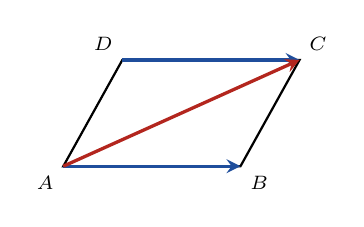
\begin{tikzpicture}[scale=0.75,font=\scriptsize,>=stealth]
\coordinate (A) at (0,0); \coordinate (B) at (3,0); \coordinate (C) at (4,1.8); \coordinate (D) at (1,1.8);
\draw[thick] (A)--(B)--(C)--(D)--cycle;
\draw[->,very thick,cDef] (A)--(B); \draw[->,very thick,cDef] (D)--(C);
\draw[->,very thick,cThm] (A)--(C);
\node[below left] at (A){$A$}; \node[below right] at (B){$B$}; \node[above right] at (C){$C$}; \node[above left] at (D){$D$};
\end{tikzpicture}\end{LTR}\par\Lab{cRem}{ملاحظات}\par\ck\ معاكس الشعاع $\overrightarrow{AB}$ هو $\overrightarrow{BA}$ ، و $\overrightarrow{AB}+\overrightarrow{BA}=\vec0$.\par
\ck\ $\overrightarrow{MA}-\overrightarrow{MB}=\overrightarrow{MA}+\overrightarrow{BM}=\overrightarrow{BA}$.\par
}{}{}
\Row{}{%
\Lab{cThm!80!black}{حذار}\ $AB+BC=AC$ (أطوال) خاطئة في الحالة العامة ؛ المساواة صحيحة للأشعة فقط.}{}{}
\Row{التقويم}{%
\Lab{cEx}{تطبيق}\par بسّط: \Num{1} $\overrightarrow{AB}+\overrightarrow{CA}+\overrightarrow{BC}$ ؛ \Num{2} $\overrightarrow{MN}-\overrightarrow{PN}+\overrightarrow{PQ}$.\par\textbf{الحل:} \Num{1} $\overrightarrow{AB}+\overrightarrow{BC}+\overrightarrow{CA}=\vec0$ ؛ \Num{2} $\overrightarrow{MN}+\overrightarrow{NP}+\overrightarrow{PQ}=\overrightarrow{MQ}$.\par\textbf{واجب منزلي:} تمارين من الكتاب المدرسي.\par\smallskip\textbf{ملاحظات حول سير الحصة:} \dotfill}{25 د}{تقويم فردي.}
\end{Sayr}
\newpage
\ModhHead{18}{1 ج م ع ت}{هندسة}{الحساب الشعاعي والمعلم}{02 سا}{جداء شعاع بعدد حقيقي}%
{\begin{itemize}\item مجموع شعاعين وعلاقة شال.\end{itemize}}%
{\begin{itemize}\item التعرّف على جداء شعاع بعدد حقيقي وإنشاؤه.\item استعمال خواص الجداء في الحساب الشعاعي.\end{itemize}}%
{المنهاج ، الكتاب المدرسي ، مراجع ، أدوات الهندسة.}
\begin{Sayr}
\Row{مرحلة الانطلاق}{%
\textbf{التهيئة النفسية:} أنشئ $\overrightarrow{AB}+\overrightarrow{AB}$ و $\overrightarrow{AB}+\overrightarrow{AB}+\overrightarrow{AB}$. كيف نكتبهما باختصار؟}{10 د}{سؤال يقود إلى الكتابة المختصرة.}
\Row{التشخيص والاكتشاف}{%
\Lab{cEx}{مناقشة نشاط 03 صفحة 252}\par\ck\ $\overrightarrow{AB}+\overrightarrow{AB}=2\overrightarrow{AB}$: نفس المنحى ونفس الاتجاه وطول مضاعف.\par
\ck\ $-2\overrightarrow{AB}$: نفس المنحى ، اتجاه معاكس ، الطول $2AB$.\par
\ck\ نقطة $M$ تحقق $\overrightarrow{AM}=\dfrac23\overrightarrow{AB}$ تقع على $[AB]$.\par
}{35 د}{عمل على ورق مرصوف.}
\Row{بناء المعارف}{%
\Lab{cDef}{تعريف}\ $k$ عدد حقيقي و $\vec u\ne\vec0$: الشعاع $k\vec u$ له نفس منحى $\vec u$ ، ونفس اتجاهه إذا كان $k>0$ وعكسه إذا كان $k<0$ ، وطوله $|k|\times\|\vec u\|$. \ و $0\vec u=\vec0$.\par\Lab{cThm}{خاصية}\ $k(\vec u+\vec v)=k\vec u+k\vec v$ ؛ $(k+k^{\prime})\vec u=k\vec u+k^{\prime}\vec u$ ؛ $k(k^{\prime}\vec u)=(kk^{\prime})\vec u$.\par}{50 د}{نرسم أمثلة لـ $k>0$ و $k<0$.}
\Row{}{%
\Lab{cEx}{مثال}\par\ck\ $I$ منتصف $[AB]$ $\iff$ $\overrightarrow{AI}=\dfrac12\overrightarrow{AB}$ $\iff$ $\overrightarrow{IA}+\overrightarrow{IB}=\vec0$.\par
\ck\ $2(\vec u-\vec v)+3\vec v-\vec u=\vec u+\vec v$.\par
\Lab{cMeth}{إنشاء نقطة}\ لإنشاء $M$ حيث $\overrightarrow{AM}=2\overrightarrow{AB}-\overrightarrow{AC}$ ننشئ $2\overrightarrow{AB}$ ثم نضيف $-\overrightarrow{AC}$ (علاقة شال).\par}{}{}
\Row{}{%
\Lab{cThm!80!black}{حذار}\ $k\vec u$ شعاع وليس عدداً.}{}{}
\Row{التقويم}{%
\Lab{cEx}{تطبيق}\par\Num{1} بسّط $3(\vec u+2\vec v)-2(\vec u-\vec v)$. \Num{2} $ABC$ مثلث: أنشئ $N$ حيث $\overrightarrow{BN}=-\dfrac12\overrightarrow{BC}$.\par\textbf{الحل:} \Num{1} $\vec u+8\vec v$.\par\textbf{واجب منزلي:} تمارين من الكتاب المدرسي.\par\smallskip\textbf{ملاحظات حول سير الحصة:} \dotfill}{25 د}{تقويم فردي.}
\end{Sayr}
\newpage
\ModhHead{19}{1 ج م ع ت}{هندسة}{الحساب الشعاعي والمعلم}{02 سا}{الارتباط الخطي لشعاعين ، التوازي والاستقامية}%
{\begin{itemize}\item جداء شعاع بعدد حقيقي.\end{itemize}}%
{\begin{itemize}\item التعرّف على شعاعين مرتبطين خطياً.\item إثبات توازي مستقيمين واستقامية ثلاث نقط.\end{itemize}}%
{المنهاج ، الكتاب المدرسي ، مراجع ، أدوات الهندسة.}
\begin{Sayr}
\Row{مرحلة الانطلاق}{%
\textbf{التهيئة النفسية:} متى تكون ثلاث نقط على استقامة واحدة؟ كيف كنا نبرهن ذلك في المتوسط؟}{10 د}{ربط بطالس وفيثاغورس.}
\Row{التشخيص والاكتشاف}{%
\Lab{cEx}{مناقشة نشاط 04 صفحة 253}\par\ck\ إذا كان $\overrightarrow{AC}=k\overrightarrow{AB}$ فإن الشعاعين لهما نفس المنحى ، والمستقيمان $(AB)$ و $(AC)$ متوازيان ويشتركان في $A$: النقط $A$ ، $B$ ، $C$ على استقامة واحدة.\par
}{35 د}{عمل ثنائي.}
\Row{بناء المعارف}{%
\Lab{cDef}{تعريف}\ نقول إن $\vec u$ و $\vec v$ \textbf{مرتبطان خطياً} إذا وُجد عدد حقيقي $k$ حيث $\vec v=k\vec u$ (أو $\vec u=\vec0$).\par\Lab{cThm}{خاصية}\par\ck\ $(AB)\parallel(CD)\iff\overrightarrow{AB}$ و $\overrightarrow{CD}$ مرتبطان خطياً.\par
\ck\ $A$ ، $B$ ، $C$ على استقامة واحدة $\iff\overrightarrow{AB}$ و $\overrightarrow{AC}$ مرتبطان خطياً.\par
}{50 د}{نكتب الطريقة على السبورة.}
\Row{}{%
\Lab{cEx}{مثال}\ $ABC$ مثلث ، $\overrightarrow{AE}=3\overrightarrow{AB}$ و $\overrightarrow{AF}=3\overrightarrow{AC}$: \ $\overrightarrow{EF}=\overrightarrow{AF}-\overrightarrow{AE}=3(\overrightarrow{AC}-\overrightarrow{AB})=3\overrightarrow{BC}$ ، إذن $(EF)\parallel(BC)$.\par\Lab{cMeth}{طريقة}\ نعبّر عن الشعاعين بدلالة شعاعين مرجعيين (باستعمال شال) ثم نقارن.\par}{}{}
\Row{}{%
\Lab{cThm!80!black}{حذار}\ شعاعان لهما نفس المنحى لا يعني أن لهما نفس الاتجاه.}{}{}
\Row{التقويم}{%
\Lab{cEx}{تطبيق}\par $ABC$ مثلث ، $M$ و $N$ حيث $\overrightarrow{AM}=\dfrac13\overrightarrow{AB}$ و $\overrightarrow{AN}=\dfrac13\overrightarrow{AC}$. بيّن أن $(MN)\parallel(BC)$.\par\textbf{الحل:} $\overrightarrow{MN}=\overrightarrow{AN}-\overrightarrow{AM}=\dfrac13\overrightarrow{BC}$.\par\textbf{واجب منزلي:} تمارين من الكتاب المدرسي.\par\smallskip\textbf{ملاحظات حول سير الحصة:} \dotfill}{25 د}{تقويم فردي.}
\end{Sayr}
\newpage
\ModhHead{20}{1 ج م ع ت}{هندسة}{الحساب الشعاعي والمعلم}{02 سا}{المعلم في المستوي: إحداثيات شعاع ، المنتصف ، المسافة ، التوازي}%
{\begin{itemize}\item الحساب الشعاعي.\item المستوي المزود بمعلم (المتوسط).\end{itemize}}%
{\begin{itemize}\item التعليم على مستقيم وفي المستوي.\item التعبير عن توازي شعاعين واستقامية ثلاث نقط في معلم.\item تغيير المبدأ.\end{itemize}}%
{المنهاج ، الكتاب المدرسي ، مراجع ، أدوات الهندسة.}
\begin{Sayr}
\Row{مرحلة الانطلاق}{%
\textbf{التهيئة النفسية:} في معلم: علّم $A(1;2)$ و $B(4;3)$. ما الانسحاب الذي يحوّل $A$ إلى $B$ ؟}{10 د}{تذكير بالمعلم.}
\Row{التشخيص والاكتشاف}{%
\Lab{cEx}{مناقشة نشاط 05 صفحة 253}\par\ck\ في معلم $(O;\vec i,\vec j)$ كل شعاع يُكتب بطريقة وحيدة $\vec u=x\vec i+y\vec j$: نكتب $\vec u(x;y)$.\par
\ck\ $\overrightarrow{AB}=(x_B-x_A)\vec i+(y_B-y_A)\vec j$: مثلاً $\overrightarrow{AB}(3;1)$.\par
}{35 د}{عمل على ورق مرصوف.}
\Row{بناء المعارف}{%
\Lab{cThm}{خاصية}\par\ck\ $\overrightarrow{AB}(x_B-x_A;y_B-y_A)$ ؛ منتصف $[AB]$: $\Big(\dfrac{x_A+x_B}2;\dfrac{y_A+y_B}2\Big)$.\par
\ck\ في معلم \textbf{متعامد ومتجانس}: $AB=\sqrt{(x_B-x_A)^2+(y_B-y_A)^2}$.\par
\ck\ $\vec u(x;y)$ و $\vec v(x^{\prime};y^{\prime})$ مرتبطان خطياً $\iff xy^{\prime}-x^{\prime}y=0$.\par
\ck\ \textbf{تغيير المبدأ:} في المعلم $(\Omega;\vec i,\vec j)$ حيث $\Omega(a;b)$: $X=x-a$ و $Y=y-b$.\par
\Lab{cEx}{مثال}\ $A(1;2)$ ، $B(4;3)$ ، $C(7;4)$: $\overrightarrow{AB}(3;1)$ و $\overrightarrow{AC}(6;2)$ ، $3\times2-1\times6=0$: النقط على استقامة واحدة ، و $AB=\sqrt{10}$.\par}{50 د}{نلخص الدساتير في جدول.}
\Row{}{%
\Lab{cThm!80!black}{حذار}\ دستور المسافة صحيح في معلم متعامد ومتجانس فقط.}{}{}
\Row{التقويم}{%
\Lab{cEx}{تطبيق}\par\Num{1} هل $\vec u(2;-3)$ و $\vec v(-4;6)$ مرتبطان خطياً؟ \Num{2} $A(1;1)$ ، $B(3;2)$ ، $C(4;5)$: عيّن $D$ حيث $ABCD$ متوازي أضلاع.\par\textbf{الحل:} \Num{1} $2\times6-(-3)(-4)=0$: نعم ؛ \Num{2} $\overrightarrow{AD}=\overrightarrow{BC}(1;3)$ ، إذن $D(2;4)$.\par\textbf{واجب منزلي:} تمارين من الكتاب المدرسي.\par\smallskip\textbf{ملاحظات حول سير الحصة:} \dotfill}{25 د}{تقويم فردي.}
\end{Sayr}
\newpage
\ModhHead{21}{1 ج م ع ت}{هندسة}{الحساب الشعاعي والمعلم}{02 سا}{معادلة مستقيم ومعامل التوجيه}%
{\begin{itemize}\item الدالة التآلفية وتمثيلها.\item إحداثيات شعاع.\end{itemize}}%
{\begin{itemize}\item التعرّف على معامل توجيه مستقيم.\item تعيين معادلة مستقيم من نقطتين أو من نقطة ومنحى.\item إنشاء مستقيم عُلمت معادلة له.\end{itemize}}%
{المنهاج ، الكتاب المدرسي ، مراجع ، أدوات الهندسة.}
\begin{Sayr}
\Row{مرحلة الانطلاق}{%
\textbf{التهيئة النفسية:} ارسم تمثيل الدالة $x\mapsto2x+1$. ما هذا التمثيل؟}{10 د}{ربط بالدالة التآلفية.}
\Row{التشخيص والاكتشاف}{%
\Lab{cEx}{مناقشة نشاط 06 صفحة 253}\par\ck\ النقطة $M(x;y)$ تنتمي إلى المستقيم $(AB)$ إذا وفقط إذا كان $\overrightarrow{AM}$ و $\overrightarrow{AB}$ مرتبطين خطياً: نحصل على علاقة بين $x$ و $y$.\par
\ck\ مثلاً $A(1;2)$ و $B(3;6)$: $(x-1)\times4-(y-2)\times2=0$ أي $y=2x$.\par
}{35 د}{عمل ثنائي.}
\Row{بناء المعارف}{%
\Lab{cThm}{خاصية}\par\ck\ كل مستقيم غير موازٍ لمحور التراتيب له معادلة من الشكل $y=mx+p$ ؛ $m$ \textbf{معامل التوجيه} و $p$ \textbf{الترتيب إلى المبدأ}.\par
\ck\ كل مستقيم موازٍ لمحور التراتيب له معادلة من الشكل $x=c$.\par
\ck\ $m=\dfrac{y_B-y_A}{x_B-x_A}$ ($x_A\ne x_B$).\par
\ck\ مستقيمان متوازيان $\iff$ لهما نفس معامل التوجيه.\par
\Lab{cEx}{مثال}\ المستقيم الذي يشمل $C(0;-1)$ ويوازي $y=2x$: \ $y=2x-1$.\par}{50 د}{نرسم عدة مستقيمات بمعاملات توجيه مختلفة.}
\Row{}{%
\Lab{cMeth}{إنشاء مستقيم}\ نعيّن نقطتين منه (مثلاً $x=0$ و $x=1$) ونصلهما.\par\Lab{cThm!80!black}{حذار}\ المستقيم $x=c$ ليس تمثيلاً لدالة.}{}{}
\Row{التقويم}{%
\Lab{cEx}{تطبيق}\par\Num{1} عيّن معادلة المستقيم الذي يشمل $E(-1;4)$ و $F(2;-2)$. \Num{2} هل $G(3;-4)$ تنتمي إليه؟\par\textbf{الحل:} \Num{1} $m=\dfrac{-2-4}{2+1}=-2$ و $4=2+p$ ، إذن $y=-2x+2$ ؛ \Num{2} $-2\times3+2=-4$: نعم.\par\textbf{واجب منزلي:} تمارين من الكتاب المدرسي.\par\smallskip\textbf{ملاحظات حول سير الحصة:} \dotfill}{25 د}{تقويم فردي.}
\end{Sayr}
\newpage
\ModhHead{22}{1 ج م ع ت}{هندسة}{الحساب الشعاعي والمعلم}{02 سا}{جملة معادلتين خطيتين لمجهولين}%
{\begin{itemize}\item معادلة مستقيم.\item حل معادلة من الدرجة الأولى.\end{itemize}}%
{\begin{itemize}\item حل جملة معادلتين خطيتين لمجهولين.\item التفسير البياني للحل.\item ترييض مشكلات.\end{itemize}}%
{المنهاج ، الكتاب المدرسي ، مراجع ، أدوات الهندسة.}
\begin{Sayr}
\Row{مرحلة الانطلاق}{%
\textbf{التهيئة النفسية:} في مزرعة دجاج وأرانب: $10$ رؤوس و $28$ رجلاً. كم دجاجة وكم أرنباً؟}{10 د}{مشكلة تقليدية مشوقة.}
\Row{التشخيص والاكتشاف}{%
\Lab{cEx}{مناقشة نشاط 07 صفحة 253}\par\ck\ نسمي $x$ عدد الدجاج و $y$ عدد الأرانب: $x+y=10$ و $2x+4y=28$.\par
\ck\ بالتعويض: $x=10-y$ ، $20-2y+4y=28$ ، $y=4$ ، $x=6$.\par
\ck\ كل معادلة هي معادلة مستقيم ، والحل هو إحداثيا نقطة تقاطعهما $(6;4)$.\par
}{35 د}{نترك التلاميذ يجربون طرقهم.}
\Row{بناء المعارف}{%
\Lab{cThm}{خاصية}\ الجملة $\begin{cases}ax+by=c\\a^{\prime}x+b^{\prime}y=c^{\prime}\end{cases}$:\par\ck\ إذا كان $ab^{\prime}-a^{\prime}b\ne0$: حل وحيد (مستقيمان متقاطعان).\par
\ck\ إذا كان $ab^{\prime}-a^{\prime}b=0$: لا حل (مستقيمان متوازيان تماماً) أو ما لا نهاية من الحلول (منطبقان).\par
\Lab{cMeth}{طرق الحل}\ التعويض ، الجمع (التركيب الخطي) ، أو الحل البياني (تقريبي).\par}{50 د}{نرسم المستقيمين بالحاسبة البيانية.}
\Row{}{%
\Lab{cEx}{مشكلة}\ تذكرتان للكبار و $3$ للصغار بـ $1300$ DA ، وتذكرة كبير و $2$ للصغار بـ $750$ DA: \ $2a+3c=1300$ و $2a+4c=1500$ ، بالطرح $c=200$ ثم $a=350$.\par\Lab{cThm!80!black}{حذار}\ نتحقق دائماً من الحل في المعادلتين.}{}{}
\Row{التقويم}{%
\Lab{cEx}{تطبيق}\par حل: \Num{1} $\begin{cases}3x-2y=4\\x+y=3\end{cases}$ \quad \Num{2} $\begin{cases}x-2y=1\\-2x+4y=3\end{cases}$\par\textbf{الحل:} \Num{1} $(2;1)$ ؛ \Num{2} $1\times4-(-2)(-2)=0$ والمستقيمان متوازيان: لا حل.\par\textbf{واجب منزلي:} تمارين حوصلة المحور من الكتاب المدرسي.\par\smallskip\textbf{ملاحظات حول سير الحصة:} \dotfill}{25 د}{نهاية المحور: فرض أو تمارين حوصلة.}
\end{Sayr}
\end{document}
